\documentclass[11pt]{article}
\usepackage[T1]{fontenc}
\usepackage[utf8]{inputenc}
\usepackage[margin=0.92in]{geometry}
\usepackage{mathptmx,amsmath,amssymb,microtype}
\usepackage{booktabs,tabularx,graphicx,xcolor,enumitem}
\usepackage{hyperref}
\definecolor{ink}{HTML}{2B342E}
\definecolor{sage}{HTML}{5E7957}
\definecolor{copper}{HTML}{B4563D}
\hypersetup{colorlinks=true,linkcolor=sage,urlcolor=sage,citecolor=sage,pdftitle={Folio: A Real-Time Jev Paper Reviewer}}
\graphicspath{{reports/}{./}}
\setlength{\parindent}{0pt}
\setlength{\parskip}{6pt}
\setlength{\emergencystretch}{2em}
\setlist[itemize]{leftmargin=1.3em,itemsep=2pt,topsep=4pt}
\newcommand{\code}[1]{\texttt{#1}}
\title{\vspace{-1.0cm}{\color{copper}\large FOLIO / RESEARCH ENGINEERING}\vspace{0.3cm}\\
\Huge A Closer Read, a Clearer Decision\\[0.3cm]
\Large A Real-Time, Section-Level Paper Reviewer Built with Jev}
\author{Application design, implementation, and validation report}
\date{19 September 2026}

\begin{document}
\maketitle
\begin{abstract}
We implement Folio, a web application that accepts research PDFs, identifies sections, streams criterion-level assessments from TypeSafe's Jev model, and calculates an inspectable overall score. The system combines four core typed judgments, with an optional fifth for venue fit grounded in retrieved website passages. Every upload starts a fresh review; cancellation and generation identifiers prevent an earlier upload from overwriting a later one. A general-review study comprises three repetitions on each of two original synthetic manuscripts and one published paper. Mean completion latency is 0.656--1.240 seconds. The structured synthetic manuscript scores 80.7/100, its deliberately vague variant 20.5/100, and the published paper 68.8/100. These scores are not validated measures of scientific merit. Two additional uploads with NeurIPS 2026 guidance complete in 1.49 and 1.14 seconds, including retrieval. The application exposes the rubric, model distributions, selected website sources, session history, and LaTeX/JSON exports.
\end{abstract}

\section{Research objective and scope}
The requested system should support an iterative research workflow: upload a manuscript, inspect feedback section by section, revise, and re-upload without manually triggering a separate scoring operation. The implementation must provide both a usable interface and an explicit account of what its numbers mean.

Folio treats assessment as a collection of narrow judgments. Jev accepts textual state and typed questions, returning structured values rather than free-form prose~\cite{introduction}. The application therefore owns extraction, weighting, arithmetic, thresholds, and feedback presentation. It does not pretend that Jev has produced a novel written rationale. The resulting product is a research-assistance prototype for a personal workspace, not a replacement for expert peer review or a calibrated acceptance predictor.

\section{Architecture and interaction}
\subsection{Application components}
The interface uses React 19, TypeScript, and Vite; a FastAPI service handles uploads and Jev calls. Locally bundled fonts, restrained sage and copper colors, and a serif reading hierarchy support a manuscript-focused interface. The main views are the review workspace, session history, and a fully inspectable rubric. The review workspace contains provisional or final score cards, a section navigator, a selected-section assessment, and the extracted manuscript.

The data path is:
\begin{center}
\small
PDF upload $\rightarrow$ text and layout extraction $\rightarrow$ section/passages\\
$\rightarrow$ concurrent Jev evaluations $\rightarrow$ streamed section results\\
$\rightarrow$ deterministic aggregation $\rightarrow$ final recommendation and exports.
\end{center}

The Python service calls \code{POST https://api.typesafe.ai/v1/systemone} with bearer authentication, a named textual state, the pinned model \code{jev-1.13.0}, and four or five Score questions~\cite{api}. The environment accepts \code{JEV\_API\_KEY} or \code{TYPESAFE\_API\_KEY}. Credentials remain on the server and are excluded from version control and client assets. The response model, rubric version, document hash, profile, token usage, elapsed time, and review identifier accompany exported reviews.

\subsection{Real-time semantics}
The upload endpoint returns newline-delimited JSON. Its events describe extraction, manuscript structure, section starts, completed section results, periodic heartbeats, terminal errors, and final completion. Up to three sections run concurrently within a review; a shared semaphore limits simultaneous Jev requests across reviews. Results appear in completion order, while the section list retains document order. The aggregate remains explicitly provisional until every section completes.

Uploading another PDF aborts the previous browser request. A monotonically increasing client generation counter prevents late callbacks from altering the current review. Server generator cleanup cancels pending section tasks and closes the HTTP client. The file input is cleared after selection so selecting the identical filename triggers another upload. No review-result cache is used. An already accepted upstream request may still be processed or billed after local cancellation.

\subsection{PDF extraction and coverage}
PyMuPDF supplies text spans, font information, and bounding boxes~\cite{pymupdf}. The parser reconstructs column order, splits blocks that contain lines from different columns, removes repeated margin labels, ignores rotated marginal text, normalizes ligatures, and recognizes typographic and numbered headings. Wrapped headings are joined. Supplementary headings are assigned an appendix role. If no headings are recognized, page-level review units are used with an explicit warning.

Inputs are bounded at 20 MB, 120 pages, 400,000 extracted characters, and 64 review units. Password-protected, damaged, and textless PDFs receive actionable errors. Long sections are divided into consecutive passages of at most 9,000 UTF-8 bytes; all extracted characters are retained. This conservative byte budget leaves room for questions and context within the documented model window~\cite{models}. Passage boundaries need not coincide with paragraphs, and local passage scoring can miss cross-passage arguments. The title, section outline, and at most 1,800 abstract characters provide supporting context; the target section itself is not silently truncated.

\section{Scoring method}
\subsection{Atomic criteria}
Each passage receives four core five-level questions. Each level has a concrete descriptive criterion, not just a numeric label. Research, survey, and theory profiles adapt what evidence and completeness reasonably require. Section-purpose instructions distinguish, for example, a concise abstract from a reproducible methods section. Manuscript text is explicitly designated as untrusted evidence; instructions inside it must not redefine the rubric. This prompting is a mitigation, not a proof of injection resistance.

\begin{table}[ht]
\centering
\caption{Core criteria and weights for a general review without venue grounding.}
\begin{tabularx}{\linewidth}{l r X}
\toprule
Criterion & Weight & Judgment \\
\midrule
Clarity & 0.20 & Whether definitions and organization communicate the passage's meaning. \\
Rigor & 0.35 & Whether reasoning is justified within explicit assumptions. \\
Evidence & 0.30 & Whether claims have specific, appropriately scoped support. \\
Completeness & 0.15 & Whether the section supplies the details required for its purpose. \\
\bottomrule
\end{tabularx}
\end{table}

For passage $c$, section $s$, criterion $d$, and level $k\in\{0,\ldots,4\}$, let $p_{scdk}$ denote Jev's returned probability. The normalized criterion score is
\begin{equation}
q_{scd}=25\sum_{k=0}^{4} k\,p_{scdk}.
\end{equation}
The HTTP response also provides this expectation directly as a Score; the implementation validates that the reported score and distribution agree within a rounding tolerance~\cite{score}. Non-finite or out-of-range values, missing answers, invalid distributions, or inconsistent scores fail closed.

If $n_{sc}$ is a passage's character count, the section criterion score and total are
\begin{equation}
q_{sd}=\frac{\sum_c n_{sc}q_{scd}}{\sum_c n_{sc}},\qquad
Q_s=\sum_d w_d q_{sd}.
\end{equation}
No model is asked to perform the arithmetic. Passage probabilities and confidence are averaged with the same character weights. Readable findings select the nearest rubric level to the averaged score; this summary can conceal a multimodal distribution, so the distribution is separately available.

\subsection{Section roles and overall score}
Role weights are abstract 5, introduction 10, related work 10, methods 25, results 25, discussion 12, conclusion 8, references 5, appendix 3, and other 10. They are relative weights normalized over roles actually present, not percentages assigned to missing sections. Let $r(s)$ be a section's role, $a_r$ its role weight, and $m_s$ its word count. Then
\begin{equation}
\alpha_s=\frac{a_{r(s)}}{\sum_{r\,\mathrm{present}}a_r}
\frac{m_s}{\sum_{j:r(j)=r(s)}m_j},\qquad
Q=\sum_s\alpha_s Q_s.
\end{equation}
Thus, splitting a role into more subsections does not itself increase that role's total influence. During streaming, the provisional total is renormalized over completed sections, while the underlying full-document weights remain fixed. Missing scientific content cannot be inferred solely from missing headings: this policy consequently cannot establish that a paper is complete at the document level.

Scores of at least 85 yield ``Strong submission''; at least 70, ``Promising; minor revisions''; at least 55, ``Major revisions suggested''; lower scores, ``Needs substantial work.'' These thresholds are design choices. If mean model confidence is below 0.45, the result becomes ``Expert review needed.'' The displayed mean is an application aggregate, not a separately calibrated confidence statistic. Incomplete reviews receive no final recommendation. Model confidence describes output concentration and is not a guarantee of correctness~\cite{confidence}.

\section{Venue-grounded review extension}
Rubric version \code{folio-1.1} adds a target venue name, official website or review-guidelines URL, and optional track/category. The interface defaults to NeurIPS 2026 and its official reviewer guidelines, with the General category selected~\cite{neurips}. Users can instead supply another conference or journal or choose a general research review. Their selected venue is retained for subsequent reviews in the same session. A preview exposes selected guidance before upload; every upload retrieves the guidance again. Changing the venue triggers a new assessment of the retained PDF, while history keeps the source context of each original review.

\textbf{Retrieval and attribution.} The service reads a public HTTPS HTML page and up to two relevant same-site links. It selects paragraphs using review-criterion and scope terms, retains nearby headings, and prioritizes the requested track; identifiable other tracks are excluded when a matching category is found. Each page contributes at most 2,400 UTF-8 bytes of selected passages. URLs, retrieval timestamps, decoded-page SHA-256 hashes, and the actual selected passages accompany the report. The model receives these passages for every section and criterion. JSON exports preserve them; LaTeX provides provenance and short excerpts. Selection is heuristic, and a supplied website's official status is not independently verified.

Website connections use validated public IP addresses with the original TLS hostname. Redirects remain on the same site; downloads are limited to 2 MB per page with a 35-second overall retrieval deadline. No manuscript text or API secret is sent to the website. Unusable root guidance stops the review before model scoring; unreadable optional linked pages generate visible warnings. Login-protected pages, JavaScript-only content, and PDF guidance are unsupported. Website text is designated as untrusted evidence, subject to the same prompt-injection caveat as manuscript text.

\textbf{Scoring.} A fifth typed judgment evaluates how the section supports a contribution aligned with the documented scientific scope and priorities. All core judgments also receive the venue context. If $v_s$ denotes the venue-fit score, the section total becomes
\begin{equation}
Q_s^{\mathrm{venue}}=0.16q_{s,\mathrm{clarity}}+0.28q_{s,\mathrm{rigor}}+
0.24q_{s,\mathrm{evidence}}+0.12q_{s,\mathrm{completeness}}+0.20v_s.
\end{equation}
The role aggregation and provisional/final semantics remain unchanged. These weights and recommendation thresholds belong to Folio; they are not an official venue scale or an estimate of acceptance probability. Selected excerpts cannot establish exhaustive policy compliance, external novelty, or full alignment with all track requirements.

\section{Validation protocol}
\subsection{Automated engineering checks}
The delivered test suite includes 72 backend checks and 24 browser scenarios across desktop and mobile configurations. Backend checks cover PDF extraction and limits, score validation, aggregation, confidence abstention, retries, cancellation, repeated uploads, and LaTeX escaping. Venue checks additionally cover public-address restrictions, pinned connections, redirect isolation, source budgets, track separation, source provenance, five-question model requests, scoring arithmetic, and retrieval failure without a false final result. Browser checks exercise incremental streams, uploads, stale results, history, exports, venue previews and changes, retained source context, focus behavior, and automated WCAG A/AA checks. Automated accessibility checks do not constitute exhaustive accessibility certification.

The engineering suite replaces the external model with fixtures; it verifies software behavior, not model accuracy. A separate study uses the configured live Jev endpoint. Production bundling and compilation of both this report and a real exported review are also checked.

\subsection{Live documents and measurements}
The original \code{folio-1.0} general-review study contains three documents, reviewed three times each under the research profile without venue grounding:
\begin{itemize}
\item \textbf{Structured synthetic manuscript:} an original three-page, eight-section example with explicit procedures and limitations. It clearly labels its numerical findings as illustrative and states that experiments were not conducted.
\item \textbf{Vague synthetic variant:} a two-page, eight-section version retaining the abstract and references but replacing six substantive bodies with unsupported assertions. It is a controlled degradation fixture, not an independent scientific paper.
\item \textbf{Published-paper layout and integration check:} the 14-page second arXiv version of \emph{On Calibration of Modern Neural Networks} by Guo et al.~\cite{guo}, with 16 detected review units including supplementary material.
\end{itemize}
The benchmark measures client wall-clock time from upload to the first section result and to completion. Model calls are real, with three-way section concurrency; no artificial speedup or precomputed review is used. Measurements were made on 19 September 2026, with Python 3.11.7, PyMuPDF 1.28.2, FastAPI 0.141.1, and HTTPX 0.28.1. They describe this environment and workload, not a latency service-level guarantee. Raw event timings and per-section scores are retained in \code{reports/benchmark-results.json}.

\section{Findings}
\begin{table}[ht]
\centering
\small
\caption{Three live reviews per document. Score spread is sample standard deviation. Latencies are arithmetic means in seconds.}
\IfFileExists{reports/measurement-table.tex}{\begin{tabular}{lrrr rr}
\toprule
Document & Pages & Units & Score $\pm$ SD & First result & Complete \\
\midrule
Structured synthetic & 3 & 8 & 80.70 $\pm$ 0.26 & 0.303 & 0.705 \\
Vague synthetic & 2 & 8 & 20.47 $\pm$ 0.06 & 0.276 & 0.656 \\
Published paper & 14 & 16 & 68.77 $\pm$ 0.15 & 0.393 & 1.240 \\
\bottomrule
\end{tabular}
}{\begin{tabular}{lrrr rr}
\toprule
Document & Pages & Units & Score $\pm$ SD & First result & Complete \\
\midrule
Structured synthetic & 3 & 8 & 80.70 $\pm$ 0.26 & 0.303 & 0.705 \\
Vague synthetic & 2 & 8 & 20.47 $\pm$ 0.06 & 0.276 & 0.656 \\
Published paper & 14 & 16 & 68.77 $\pm$ 0.15 & 0.393 & 1.240 \\
\bottomrule
\end{tabular}
}
\end{table}

\begin{figure}[ht]
\centering
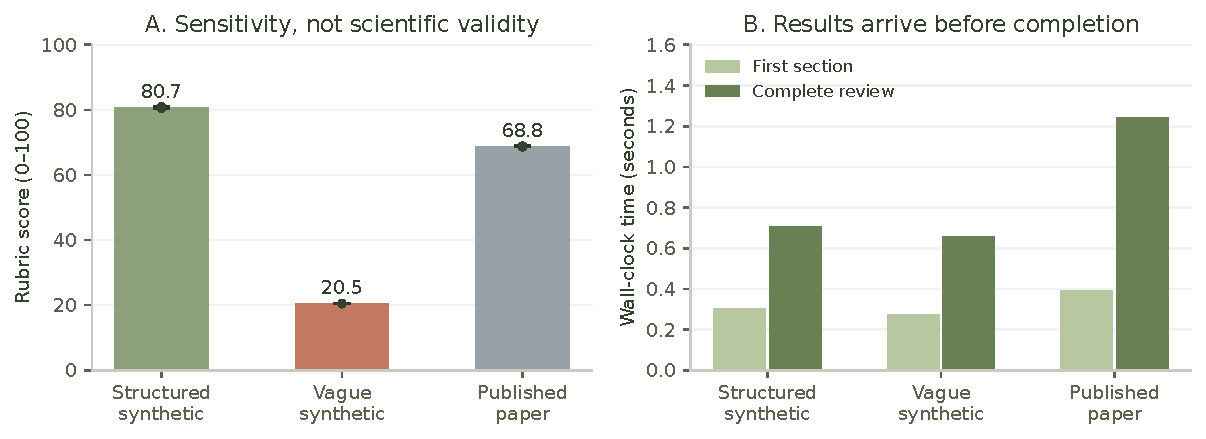
\includegraphics[width=\linewidth]{benchmark-figure.pdf}
\caption{Recorded model scores and stream latencies. Three repeat measurements per document are insufficient to establish generalization or scientific-review validity.}
\end{figure}

\textbf{Responsiveness.} The first feedback arrived in approximately 0.28--0.39 seconds on average. The longer published document completed in approximately 1.24 seconds. All nine live streams delivered every extracted review unit and a final result. Each synthetic review used 11,830 or 11,444 input tokens, while the published-paper review used 43,248 input tokens. These are summed across multiple requests, not a single-request context length.

\textbf{Controlled sensitivity.} The structured and vague fixtures differ by approximately 60.2 score points. Repeat standard deviations were about 0.26 and 0.06 points respectively. This indicates stability for these exact inputs and sensitivity to deliberately removed detail. It provides no estimate of agreement with human reviewers, susceptibility to subtler manipulation, or reliability across disciplines.

\textbf{Scientific-validity limitation.} The structured synthetic example scored above the actual published paper despite explicitly stating that its results were invented for demonstration. Its score therefore cannot be interpreted as evidence that a scientific contribution was established. Conversely, the published paper's lower score is not an expert reassessment of that paper. Extraction artifacts, graphical evidence, local context, role classification, and generic criteria plausibly affect the result, but this study does not isolate those causes. The interface accordingly presents these outputs as rubric assessments and avoids an automatic venue-acceptance decision.

\textbf{Parsing matters.} Initial inspection exposed a rotated arXiv stamp being mistaken for a title, table entries being treated as headings, and horizontally merged text blocks disrupting column order. Regression checks led to corrections in each case. The final parser recognizes the correct title, retains numeric table text without promoting it to headings, and combines wrapped supplementary headings. These improvements do not establish correctness on arbitrary mathematical, multilingual, or irregular-layout PDFs.

\subsection{Live venue-grounding integration check}
Two further uploads of the structured synthetic manuscript used \code{folio-1.1}, the research profile, and the NeurIPS 2026 General reviewer-guidelines preset. Each fetched one source page, selected four passages, and completed all eight sections with five criterion scores. Both totals were 77.4/100; venue-fit aggregates were 65.2 and 65.9. First-section feedback arrived at 1.133 and 0.774 seconds, with completion at 1.487 and 1.140 seconds. These times include current website retrieval, unlike the general-review timings above. The uploads generated distinct review identifiers and fresh source timestamps. Raw events and provenance are retained in \code{reports/venue-validation.json}; an exported assessment is in \code{reports/venue-example-review.tex}.

This verifies retrieval, model integration, aggregation, repeat uploads, and source export on one venue and one synthetic paper. It does not establish whether venue grounding improves expert agreement. Neither the venue-fit values nor the score change from the earlier general review should be interpreted as a measured probability of acceptance or a causal estimate of improved review quality.

\section{Operational and research limitations}
\begin{itemize}
\item \textbf{No external verification.} Jev receives extracted text, not rendered figures or an external literature search. Novelty, citation validity, numerical correctness, and proof validity remain unverified. Image-only pages require OCR beforehand.
\item \textbf{No calibrated quality scale.} The four core dimensions, optional venue-fit dimension, role weights, confidence thresholds, and recommendation boundaries have not been fitted to held-out expert reviews. Averaging can hide a severe local failure; the interface exposes section details for that reason.
\item \textbf{Bounded local reasoning.} A 9,000-byte passage may cut across a logical argument. The abstract context is bounded. Long-range consistency and completeness of an entire proof or experimental program are not established.
\item \textbf{Adversarial input.} Jev's documented limitations include sensitivity to adversarial state, numerical reasoning, and distracting context~\cite{jaggedness}. Explicit rubric instructions reduce ambiguity, but adversarial robustness was not established by this study.
\item \textbf{Privacy and deployment.} Upload buffering may use temporary files, which are closed after reading. Folio retains no server-side manuscripts or reports; the browser retains up to 20 completed reviews in memory. Text is still processed by TypeSafe under its own policies. Public deployment requires authentication, quotas, and proxy-level upload controls beyond this personal-workspace prototype.
\item \textbf{Feedback provenance.} Findings and revision prompts are templates selected from the implemented rubric, not generated expert explanations. Opening excerpts are contextual, not asserted causal evidence for model judgments. Non-ASCII text is normalized for portable LaTeX export; JSON retains exact Unicode.
\end{itemize}

\section{Reproducibility and next research steps}
The repository contains pinned dependency lockfiles, the full rubric, unit/integration/browser tests, the benchmark script, raw live measurements, a generated example review, and the LaTeX source for this report. Run \code{npm run dev} to open the local interface; run \code{npm test} and \code{npm run test:e2e} for engineering validation. With the server running, \code{uv run python scripts/benchmark.py --public} repeats the live study and uses the configured API credential.

Run \code{uv run python scripts/benchmark\_venue.py} to repeat the two-upload venue check. It accepts custom venue, website, and track arguments. Repeated runs can differ because both model outputs and website contents may change; the recorded source snapshots identify what was used.

A defensible research evaluation would next collect independently reviewed manuscripts across fields, blind the reviewers to model output, define section-level ground truth, split calibration and test sets, and measure ranking agreement, error types, confidence calibration, and subgroup variation. It should compare text-only extraction with figure-aware reading, assess rubric/profile sensitivity, and test adversarial manuscripts and severely flawed yet polished papers. Until those checks are completed, Folio is best used to organize revision questions and make assumptions visible.

\begin{thebibliography}{9}
\bibitem{introduction} TypeSafe AI. \emph{Introduction}. Accessed 19 September 2026. \url{https://docs.typesafe.ai/introduction}.
\bibitem{api} TypeSafe AI. \emph{HTTP API Reference}. Accessed 19 September 2026. \url{https://docs.typesafe.ai/api}.
\bibitem{score} TypeSafe AI. \emph{Score}. Accessed 19 September 2026. \url{https://docs.typesafe.ai/primitives/score}.
\bibitem{confidence} TypeSafe AI. \emph{Confidence}. Accessed 19 September 2026. \url{https://docs.typesafe.ai/confidence}.
\bibitem{models} TypeSafe AI. \emph{Models}. Accessed 19 September 2026. \url{https://docs.typesafe.ai/models}.
\bibitem{jaggedness} TypeSafe AI. \emph{Jev 1.13 Jaggedness}. Accessed 19 September 2026. \url{https://docs.typesafe.ai/model-jaggedness/jev-1.13}.
\bibitem{pymupdf} PyMuPDF. \emph{Text Extraction Documentation}. Accessed 19 September 2026. \url{https://pymupdf.readthedocs.io/en/latest/recipes-text.html}.
\bibitem{guo} C. Guo, G. Pleiss, Y. Sun, and K. Q. Weinberger. \emph{On Calibration of Modern Neural Networks}. ICML, PMLR 70, 1321--1330, 2017. arXiv:1706.04599v2. \url{https://arxiv.org/abs/1706.04599v2}.
\bibitem{neurips} NeurIPS. \emph{NeurIPS 2026 Reviewer Guidelines}. Accessed 19 September 2026. \url{https://neurips.cc/Conferences/2026/ReviewerGuidelines}.
\end{thebibliography}
\end{document}
